%%%%%%%%%%%%%%%%%%%%%%%%%%%%% Define Article %%%%%%%%%%%%%%%%%%%%%%%%%%%%%%%%%%
\documentclass{article}
%%%%%%%%%%%%%%%%%%%%%%%%%%%%%%%%%%%%%%%%%%%%%%%%%%%%%%%%%%%%%%%%%%%%%%%%%%%%%%%

%%%%%%%%%%%%%%%%%%%%%%%%%%%%% Using Packages %%%%%%%%%%%%%%%%%%%%%%%%%%%%%%%%%%
\usepackage{geometry}
\usepackage{graphicx}
\usepackage{amssymb}
\usepackage{amsmath}
\usepackage{amsthm}
\usepackage{empheq}
\usepackage{mdframed}
\usepackage{booktabs}
\usepackage{lipsum}
\usepackage{graphicx}
\usepackage{color}
\usepackage{psfrag}
\usepackage{pgfplots}
\usepackage{bm}
\usepackage{wrapfig}
\usepackage{parskip}
%%%%%%%%%%%%%%%%%%%%%%%%%%%%%%%%%%%%%%%%%%%%%%%%%%%%%%%%%%%%%%%%%%%%%%%%%%%%%%%

% Other Settings

%%%%%%%%%%%%%%%%%%%%%%%%%% Page Setting %%%%%%%%%%%%%%%%%%%%%%%%%%%%%%%%%%%%%%%
\geometry{a4paper}

%%%%%%%%%%%%%%%%%%%%%%%%%% Define some useful colors %%%%%%%%%%%%%%%%%%%%%%%%%%
\definecolor{ocre}{RGB}{243,102,25}
\definecolor{mygray}{RGB}{243,243,244}
\definecolor{deepGreen}{RGB}{26,111,0}
\definecolor{shallowGreen}{RGB}{235,255,255}
\definecolor{deepBlue}{RGB}{61,124,222}
\definecolor{shallowBlue}{RGB}{235,249,255}
%%%%%%%%%%%%%%%%%%%%%%%%%%%%%%%%%%%%%%%%%%%%%%%%%%%%%%%%%%%%%%%%%%%%%%%%%%%%%%%

%%%%%%%%%%%%%%%%%%%%%%%%%% Define an orangebox command %%%%%%%%%%%%%%%%%%%%%%%%
\newcommand\orangebox[1]{\fcolorbox{ocre}{mygray}{\hspace{1em}#1\hspace{1em}}}
%%%%%%%%%%%%%%%%%%%%%%%%%%%%%%%%%%%%%%%%%%%%%%%%%%%%%%%%%%%%%%%%%%%%%%%%%%%%%%%

%%%%%%%%%%%%%%%%%%%%%%%%%%%% English Environments %%%%%%%%%%%%%%%%%%%%%%%%%%%%%
\newtheoremstyle{mytheoremstyle}{3pt}{3pt}{\normalfont}{0cm}{\rmfamily\bfseries}{}{1em}{{\color{black}\thmname{#1}~\thmnumber{#2}}\thmnote{\,--\,#3}}
\newtheoremstyle{myproblemstyle}{3pt}{3pt}{\normalfont}{0cm}{\rmfamily\bfseries}{}{1em}{{\color{black}\thmname{#1}~\thmnumber{#2}}\thmnote{\,--\,#3}}
\theoremstyle{mytheoremstyle}
\newmdtheoremenv[linewidth=1pt,backgroundcolor=shallowGreen,linecolor=deepGreen,leftmargin=0pt,innerleftmargin=20pt,innerrightmargin=20pt,]{theorem}{Theorem}[section]
\theoremstyle{mytheoremstyle}
\newmdtheoremenv[linewidth=1pt,backgroundcolor=shallowBlue,linecolor=deepBlue,leftmargin=0pt,innerleftmargin=20pt,innerrightmargin=20pt,]{definition}{Definition}[section]
\theoremstyle{myproblemstyle}
\newmdtheoremenv[linecolor=black,leftmargin=0pt,innerleftmargin=10pt,innerrightmargin=10pt,]{problem}{Problem}[section]
%%%%%%%%%%%%%%%%%%%%%%%%%%%%%%%%%%%%%%%%%%%%%%%%%%%%%%%%%%%%%%%%%%%%%%%%%%%%%%%

%%%%%%%%%%%%%%%%%%%%%%%%%%%%%%% Plotting Settings %%%%%%%%%%%%%%%%%%%%%%%%%%%%%
\usepgfplotslibrary{colorbrewer}
\pgfplotsset{width=8cm,compat=1.9}
%%%%%%%%%%%%%%%%%%%%%%%%%%%%%%%%%%%%%%%%%%%%%%%%%%%%%%%%%%%%%%%%%%%%%%%%%%%%%%%

%%%%%%%%%%%%%%%%%%%%%%%%%%%%%%% Title & Author %%%%%%%%%%%%%%%%%%%%%%%%%%%%%%%%
\title{\textbf{Operating Systems CS/CE 232L/324L}\\ \textbf{Lab 02}}
\author{Ali Muhammad Asad \\ aa07190}
\date{} %Leave uncommented if u want automatic date which is done through maketitle, else u can uncomment this and type anything else u want over here - not necessary to enter a date over here
%%%%%%%%%%%%%%%%%%%%%%%%%%%%%%%%%%%%%%%%%%%%%%%%%%%%%%%%%%%%%%%%%%%%%%%%%%%%%%%

\begin{document}
\maketitle
    
{\Large \textbf{\underline{Exercises:}}}

\noindent\textbf{Prompt:} Create a text file with at least three columns and ten lines. Name it as your student ID, and have dummy data in the file, however, the third column should be integer values.

Command: \texttt{touch aa07190.txt} \\ The above command creates a txt file, and then the file can be opened in a text editor and updated accordingly.

Command: \texttt{nano aa07190.txt} \\ This command creates and opens the txt file in the terminal where changes can be made

Dummy data: \\ `` \\
\begin{tabular}{c c c}
    Column1 & Column2 & Column3 \\
    value1 & valueA & 1 \\
    value2 & valueB & 2 \\
    value3 & valueC & 3 \\
    value4 & valueD & 4 \\
    value5 & valueE & 5 \\
    value6 & valueF & 6 \\
    value7 & valueG & 7 \\
    value8 & valueH & 8 \\
    value9 & valueI & 9 \\
    value0 & valueJ & 10 \\
\end{tabular} \\
''

\textbf{\underline{Tasks:}}

\textbf{1)} Change the permissions of your newly created dummy data file to enable read and write access for \texttt{others} set of people. \\ 
Ans: \texttt{chmod o+rw aa07190.txt} \\
The above command changes the permissions of the file to allow read and write access to others. `chmod' is the command to change file permissions, `o' stands for others, and `+rw' stands for read and write access where `r' is read and `w' is write.

\pagebreak
\textbf{2)} Show the first three lines of your dummy data file. \\
Ans: \texttt{head -n 3 aa07190.txt}
\begin{figure}[htbp]
    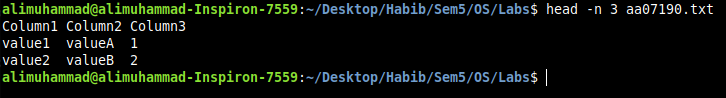
\includegraphics[width=1.0\textwidth]{lab2_2.png}
\end{figure} \\ 
The `head' command displays the head of the file, and the rest displays the first 3 lines of the file.

\vspace*{10mm}
\textbf{3)} Show the last four lines of your dummy data file. \\
Ans: \texttt{tail -n 4 aa07190.txt}
\begin{figure}[htbp]
    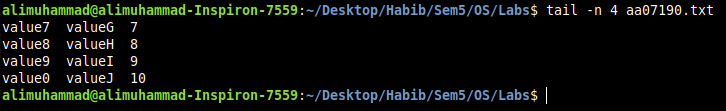
\includegraphics[width=1.0\textwidth]{lab2_3.png}
\end{figure} \\
The `tail' command displays the tail of the file, and the rest displays the last 4 lines of the file.

\vspace*{10mm}
\textbf{4)} Show the sixth line of your dummy data file. \\
Ans: \texttt{sed -n `6p' aa07190.txt}
\begin{figure}[htbp]
    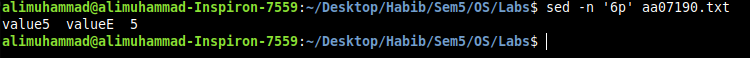
\includegraphics[width=1.0\textwidth]{lab2_4.png}
\end{figure}

\pagebreak
\textbf{5)} Display the third column of your dummy data file. \\
Ans: \texttt{cut -f 3 aa07190.txt} \\ Alternatively we can also use: \\ \texttt{awk `$\{\text{print } \$3\}$' aa07190.txt}

Both commands print or extract the third field / column from the .txt file. The display for both the commands is as follows:
\begin{figure}[htbp]
    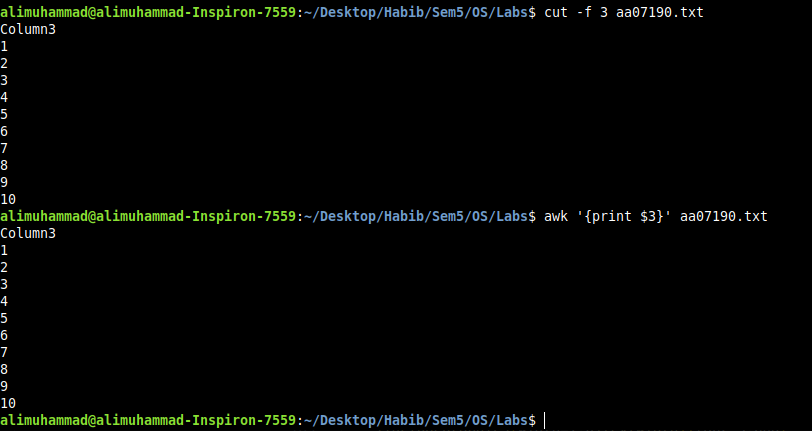
\includegraphics[width=1.0\textwidth]{lab2_5.png}
\end{figure}

\vspace*{10mm}
\textbf{6)} Display the first column of your dummy data file in sorted order. \\
Ans: \texttt{cut -f 1 aa07190.txt $|$ sort} \\
The above command first extracts the first column from the .txt file and then sorts it. 
\begin{figure}[htbp]
    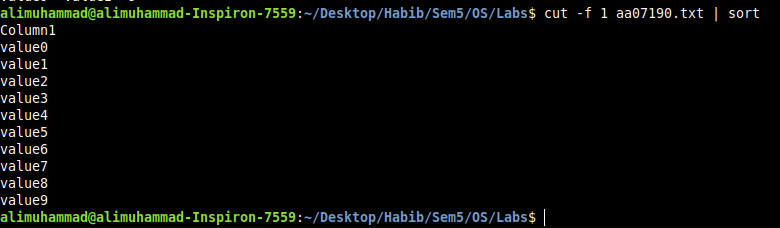
\includegraphics[width=1.0\textwidth]{lab2_6.png}
\end{figure}

\pagebreak
\textbf{7)} Display the maximum value in the third column of your data file. \\
Ans: \texttt{cut -f 3 aa07190.txt $|$ sort -n $|$ tail -n 1} \\ Alternatively: \\ \texttt{cut -f 3 aa07190.txt $|$ sort -n -r $|$ head -n 1} \\
Both the commands give the maximum value in the third column. The first command sorts in ascending order, and then `tail' is used to extract the first element from the tail. The second command sorts in descending order and the first element is extracted from the head.
\begin{figure}[htbp]
    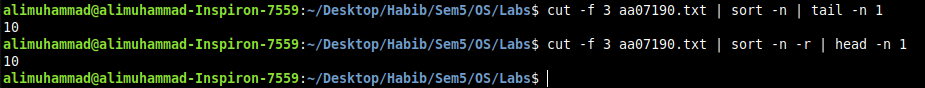
\includegraphics[width=1.0\textwidth]{lab2_7.png}
\end{figure}

\vspace*{10mm}
\textbf{8)} Obtain the number of words in your dummy data file, and store them in another file (name it count.txt). \\ Do this in a single command. \\
Ans: \texttt{wc -w < aa07190.txt > count.txt} \\
The `wc -w' counts the number of words in the dummy data file. `$<$' redirects the contents of the dummy data file to `wc' and `$>$' redirects the output of `wc' which is the word count to the count.txt file.
\begin{figure}[htbp]
    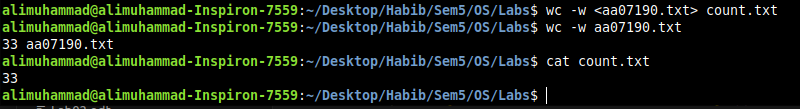
\includegraphics[width=1.0\textwidth]{lab2_8.png}
\end{figure} \\
After running the command, we can see that there were 33 words in our dummy data file, and the count.txt file has been created containing the word count.

\vspace*{10mm}
\textbf{9)} In \texttt{count.txt} append the number of characters in your dummy data file. Do this in a single command. \\
Ans: \texttt{wc -c < aa07190.txt >> count.txt} \\
The `wc -c' counts the number of characters in the file, then similarly the $<$ redirects the contents of the dummy data file to `wc' and $>>$ redirects and appends the output of `wc' which is the character count to the count.txt file.
\begin{figure}[htbp]
    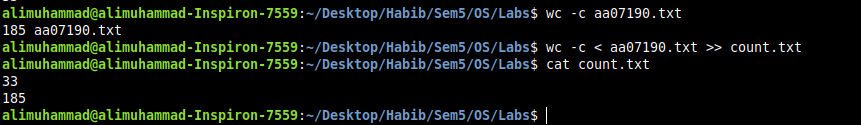
\includegraphics[width=1.0\textwidth]{lab2_9.png}
\end{figure}

\pagebreak
\textbf{10)} Display the second column of your dummy data file in reverse order $($not in alphabetical terms$)$ and store it in another file $($name it \texttt{reverse.txt}$)$. Use piping to do this in one command. \\
Ans: Since we know `tac' is the `cat' command in reverse, we can simply use `cut' to extract the second column and use `tac' to reverse the order. \\ We can use the following command: \\ \texttt{cut -f 2 aa07190.txt $|$ tac > reverse.txt} 
\begin{figure}[htbp]
    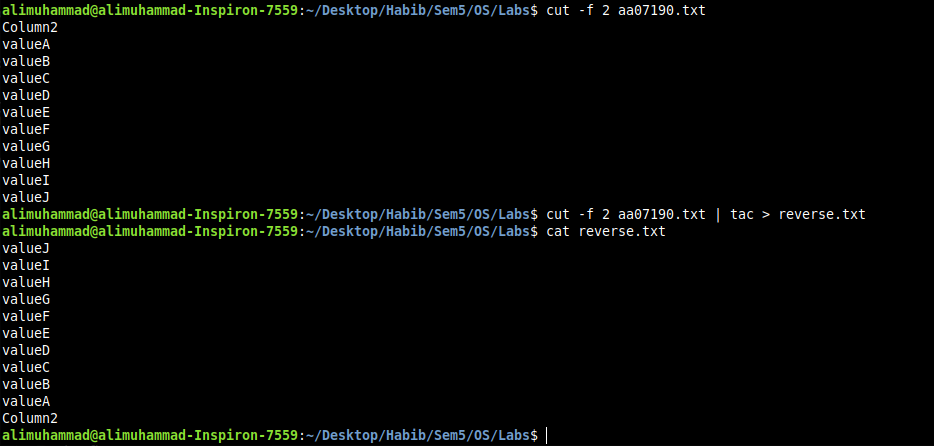
\includegraphics[width=1.0\textwidth]{lab2_10.png}
\end{figure}

The contents of the \texttt{reverse.txt} file can be seen to have been reversed as compared to the second column of our dummy data file.

\vspace*{10mm}
\textbf{11)} Display the first letter of each text value in the first column of your dummy file. Use piping to do this in one command. \\ 
Ans: \texttt{cut -c 1 aa07190.txt $|$ cut -c 1} \\
The first \texttt{cut -c 1 aa07190.txt} extracts the first character of each line in the first column, and the second \texttt{cut -c 1} extracts the first character of each line in the output of the first \texttt{cut} command. Therefore, we get the first letter of each text value in the first column of our dummy data file as shown below:
\begin{figure}[htbp]
    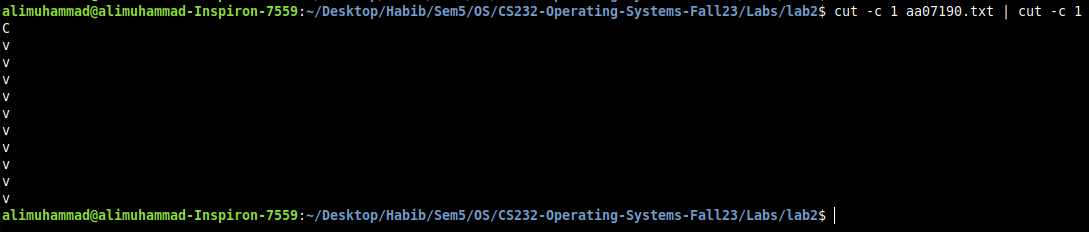
\includegraphics[width=1.0\textwidth]{lab2_11.png}
\end{figure}

\end{document}